\documentclass[12pt,a4paper]{report}

% Packages
\usepackage{times}              % Times New Roman font
\usepackage{setspace}           % Line spacing
\usepackage[a4paper, left=1.5in, right=1in, top=1in, bottom=1in]{geometry}
\usepackage{titlesec}           % Chapter/section formatting
\usepackage{fancyhdr}           % Header/Footer
\usepackage{graphicx}           % Figures
\usepackage{hyperref}           % Hyperlinks
\usepackage{tocloft}            % TOC formatting
\usepackage{lipsum}             % Dummy text (remove for real content)
\usepackage{titlesec}
\usepackage{etoolbox} % needed for patching TOC entries
\usepackage{xcolor}
\usepackage{tabularx}
\usepackage{booktabs}
\usepackage{csquotes}
\usepackage[style=ieee,backend=biber]{biblatex}
\addbibresource{citations.bib}


% Line spacing
\onehalfspacing
\setlength{\headheight}{15pt}

% Title formatting
\titleformat{\chapter}[hang]{\bfseries\centering\LARGE}{Chapter \thechapter}{1em}{}
\titleformat{\section}[hang]{\bfseries\Large}{\thesection}{1em}{}

\newcommand{\projecttitle}{Proactive Multi-Agent Orchestration for Intelligent Engagement on Education}

\newcommand{\groupnumber}{22}

\newcommand{\firststudentname}{Prakrithi Jain}
\newcommand{\firststudentusn}{1BM23CS239}

\newcommand{\secondstudentname}{Sai Pranav Enjeti}
\newcommand{\secondstudentusn}{1BM23CS286}

\newcommand{\thirdstudentname}{Shashank Shantharam Nayak}
\newcommand{\thirdstudentusn}{1BM23CS313}

\newcommand{\fourthstudentname}{Siddharth Arya}
\newcommand{\fourthstudentusn}{1BM23CS328}

\newcommand{\guide}{Shreevatsa D S}
\newcommand{\guidedesignation}{Assistant Professor}

% Fancy Header/Footer
\pagestyle{fancy}
\fancyhf{}
\lhead{\textit{\projecttitle}}
\lfoot{\textit{Dept. of CSE, BMSCE}}
\rfoot{\textit{Page \thepage}}

% Make chapter pages use fancy style
\makeatletter
\let\ps@plain\ps@fancy
\makeatother

\hyphenpenalty=10000
\exhyphenpenalty=10000
\sloppy

\begin{document}

% ---------- FRONT MATTER: ROMAN NUMBERS ----------
\pagenumbering{roman}
\setcounter{page}{1}

% ----- Title Page -----
\begin{titlepage}
  \thispagestyle{empty}
  \centering

  {\Huge \textbf{\projecttitle}}\\[1.0cm]
  
\includegraphics[width=0.18\linewidth]{VTU-Logojpg.jpg}\\[0.9cm]
  {\Large \textbf{PROJECT REPORT}}\\[0.2cm]
  {\large \textit{Submitted by}}\\[0.5cm]
  {\large Group Number: \groupnumber}\\ [0.3cm]
  {\large \firststudentname\ (\firststudentusn)}\\
  {\large \secondstudentname\ (\secondstudentusn)}\\
  {\large \thirdstudentname\ (\thirdstudentusn)}\\
  {\large \fourthstudentname\ (\fourthstudentusn)}\\[0.7cm]
  {\itshape in partial fulfillment for the award of the degree of}\\[0.15cm]
  {\Large \textbf{BACHELOR OF ENGINEERING}}\\[0.2cm]
  {\large in}\\[0.2cm]
  {\Large \textbf{COMPUTER SCIENCE AND ENGINEERING}}\\[0.9cm]
  {\large Under the Guidance of}\\
  {\large \textbf{\guide}}\\
  {\large \guidedesignation, Department of CSE, BMSCE}
  \vfill
  
\includegraphics[width=0.18\linewidth]{bmscelogo.jpg}\\[0.5cm]
  {\Large \textbf{B.M.S. COLLEGE OF ENGINEERING}}\\
  {\large (Autonomous Institution under VTU)}\\
  {\large BENGALURU - 560019}\\
  {\large Academic Year - 2025–2026}

\end{titlepage}


% ----- Certificate -----
\chapter*{Certificate}
\thispagestyle{empty}
\vspace{2cm}
This is to certify that the project report entitled \textbf{\enquote{\projecttitle}} is a bonafide work carried out by \textbf{
	\firststudentname\ (\firststudentusn),
	\secondstudentname\ (\secondstudentusn),
	\thirdstudentname\ (\thirdstudentusn),
	\fourthstudentname\ (\fourthstudentusn)
} in partial fulfillment of the requirements for the award of the degree of \textbf{Bachelor of Engineering} in \textbf{Computer Science and Engineering}, under my supervision during the academic year 2025–2026.

\vspace{2cm}
\begin{flushleft}
Guide Signature\hspace{30mm} HoD signature \hspace{25mm} Principal Signature\\
(\guide) \hspace{25mm} Dr. Kavitha Sooda \hspace{19mm} Dr. Bheemsha Arya 
\end{flushleft}
\vspace{2cm}
\begin{flushleft}
Name and signature of Examiners along with date \\
\vspace {1cm}
Examiner 1 \\
\vspace {1cm}
Examiner 2 \\
    
\end{flushleft}


%-------------Declaration ----------
\chapter*{DECLARATION}
\thispagestyle{empty}
We, hereby declare that the Major Project Phase-1 work entitled \enquote{\projecttitle} is a bonafide work and has been carried out  by us under the guidance of \guide, \guidedesignation, Department of  Computer Science and Engineering, B.M.S. College of Engineering, Bengaluru, in partial  fulfillment of the requirements of the degree of Bachelor of Engineering in Computer Science  and Engineering of Visvesvaraya Technological University, Belagavi. 
We further declare that, to the best of our knowledge and belief, this project has not been submitted either in part or in full to any other university for the award of any degree. 
\vspace{0.3cm}
\begin{flushleft}
Candidate details: 
\end{flushleft}
\vspace{0.1cm}
\begin{center}
\begin{tabular}{|c|l|c|c|}
\hline
\textbf{SL. NO.} & \textbf{Student Name} & \textbf{USN} & \textbf{Student’s Signature} \\
\hline
1 & \firststudentname & \firststudentusn & \\
\hline
2 & \secondstudentname & \secondstudentusn & \\
\hline
3 & \thirdstudentname & \thirdstudentusn & \\
\hline
4 & \fourthstudentname & \fourthstudentusn & \\
\hline
\end{tabular}
\end{center}
\begin{flushleft}
Place: Bengaluru \\
Date: \\
\end{flushleft}
Certified that these candidates are students of Computer Science and Engineering Department  of B.M.S. College of Engineering. They have carried out the project work of titled \enquote{\projecttitle} as Major Project Phase-1  work. It is in partial fulfillment for completing the requirement for the award of B.E. degree by VTU. The work is original and I duly certify the same.  
\vspace{1cm}
\begin{flushleft}
Guide Name: \\
Date: \\
Signature: \\ 
\end{flushleft}
% ----- Acknowledgment -----
\chapter*{Acknowledgment}
\thispagestyle{empty}
We extend our heartfelt appreciation to the Management of BMS College of Engineering and our Principal for offering us the necessary support and facilities for our educational pursuits.

We thank Dr. Kavitha Sooda, Head of the Department, Computer Science and Engineering, for her continual support and for allowing us to conduct this project through the usage of the unique computing facilities provided by the department.

We extend our sincere gratitude to Dr. Nandhini Vineeth and other distinguished members of the review panel. The valuable technical suggestions and reviews made by them helped us in developing the project from a mere idea to a full-fledged project.

We are also grateful to our guide \guide { }for his valuable contributions during the development of this project.
Finally, we thank all our family members, friends, and people who have directly or indirectly helped us in completing this project.
\newpage


% ----- TOC, LoF, LoT -----
\tableofcontents
\thispagestyle{empty}
\newpage
\listoffigures
\thispagestyle{empty}
\newpage
\listoftables
\thispagestyle{empty}

% ----- Abstract -----
\chapter*{Abstract}
\thispagestyle{empty}
% Write your abstract here. This should summarize the entire project including objectives, methods, and outcomes. It should be complete one full page.



% ---------- MAIN MATTER: ARABIC NUMBERS ----------

\clearpage
\pagenumbering{arabic}
\setcounter{page}{1}

% ----- Chapters -----
\chapter{Introduction}

\section{Overview}
Contemporary learning systems are changing from a passive approach to an active one with the assistance of Artificial Intelligence. In the study, we present an Intelligent Tutoring System (ITS) using a Multi-Agent Architecture. The proposed system consists of a multiple agents rather than employing a single chatbot. These agents are designed to simulate a one-on-one tutoring session like a private tutor.

\section{Motivation}
The divide in education technology is no longer just about having access to the internet; it is also about having access to quality, personalized education. E-learning systems have been used traditionally as content management systems but fail to address the Two Sigma Problem \cite{bloom1984}, whereby students receiving individual tutoring outperform those taught in classrooms. We are motivated to provide personalized education by means of autonomous agents that will be able to remember the learner’s past, understand what they upload, and help them when problems arise.

\section{Objectives}
Our main goal is to create a system that adheres to the following objectives:
\begin{itemize}
	\item Contextual Intelligence: Build an LLM Orchestration Layer that manages state across sessions using cache and long-term vector memory.
	\item Autonomous Assessment: Create a pipeline that converts raw media (documents, images, videos) into chunked information and generates evaluative questions based on the document.
	\item Automated Feedback: Create a feedback mechanism that produces reports and learning insights based on existing progress in a topic.
	\item Behavioral Persistence: Design a profiling engine that stores information about the users and their knowledge gaps. This ensures a reduction in the loss of context for the LLM.
\end{itemize}

\section{Scope}
The current study is concentrated on developing a backend system based on the above objectives.

The system will consist of an API Gateway that ensures secure communication,a data layer based on Vector Databases, and an orchestration layer, where different LLMs will fulfill various functions.

\section{SDG Justification}
This project supports United Nations Sustainable Development Goal 4 (Quality Education), SDG 9 (Industry, Innovation and Infrastructure) and SDG 10 (Reduced Inequalities). By using automation for working on time-consuming tasks such as progress tracking, the system offers an affordable, impctful solution for learners worldwide. It tries to balance the inequalities of society in obtaining quality education by providing a personalized learning companion that is available around the clock. Traditional tutoring services can be costly, posing challenges for learners in low-income communities. To alleviate this, the proposed system provides personalized tutoring capabilities that can be accessed anywhere and anytime.

\section{Existing System}
Current Learning Management Systems (LMS) are mostly static. They may not understand the state of mind of the learner, because they cannot perform one-on-one tutoring. MOOC platforms can only imitate classroom-based learning in an online setting.

Thus, current systems struggle to maintain a coherent conversation over prolonged study periods.

\section{Proposed System}
We propose that a Multi-Agent Orchestration system be adopted. In the center of this system, an LLM Orchestrator will direct user inputs towards specific agents according to their intents.

\begin{itemize}
	\item The Content Analysis Agent is concerned with parsing of documents, which are needed for processing of study materials.
	\item The Profiling Agent updates the persistent User Profile Database, accounting for the progress that the learner makes.
	\item The Question Generation Agent aligns the content with the level of difficulty of the user.
    \item The Insight Agent recommends the following actions.
    \item The Proactive Agent interacts with the user via a scheduling capability.
\end{itemize}

\section{Work Plan}
The process of implementation is planned to follow the following stages:

\begin{enumerate}
	\item Stage I: Interagent communication and storage schemas of user data development.
	\item Stage II: The creation of the API Gateway and Orchestrator.
	\item Stage III: Specialized agents' and Vector Database's development and calibration.
	\item Stage IV (Improvement): Implementation of the Proactive Scheduler and testing of the system as a whole.
\end{enumerate}

\chapter{Literature Survey}
Education has significantly evolved in the years of past, from physical attendance to Massive Online Open Courses(MOOC). With online platforms being increasingly used to learn new concepts, it has become a classic "Two Sigma Problem" \cite{bloom19842}

\section{Overview}

\section{Detailed Survey}

\section{Research Gap Identification}

\section{Mapping of Objective with Research Gap Identification} 



\chapter{Software and Hardware Requirement Specification}
For the successful implementation of an AI-enabled education system, it is important to develop a solid technical base which balances out the need for high-performance training and low-weight production. This chapter discusses the technical requirements needed for supporting the multi-agent system and the LLM-based pipeline.

\section{Functional Requirements}
In order to meet the goals relating to SDG 4, 9, and 10, the system will adhere to the following key functionalities:
\begin{itemize}
	\item \textbf{Real-time Tutoring:} The system will provide instant responses to students' queries by deploying agents that utilize large language models (LLMs).
	\item \textbf{Personalized Learning Paths:} The multi-agent architecture will evaluate student learning outcomes and modify the complexity of the learning content accordingly.
	\item \textbf{User Profiling:} The system will keep track of the activities of users in every session, ensuring that there is always a current profile. 
	\item \textbf{Information Retrieval:} he system will provide a function that allows for searching for and retrieving relevant information using vector-based search queries.
\end{itemize}

\section{Non-functional Requirements}
\begin{itemize}
	\item \textbf{Scalability:} The software architecture must be able to handle an increase in the number of simultaneous users without sacrificing performance.
	\item \textbf{Latency:} For an efficient learning experience, the agent latency must, wherever possible, remain below two seconds.
	\item \textbf{Availability:} The production environment will be accessible through Internet connectivity and have limited downtime.
	\item \textbf{Cost Efficiency:} The development process will employ open-source architectures and cloud computing systems that can be supported by free-tier accounts.
\end{itemize}

\section{Hardware Requirements}
Hardware requirements are categorized into two different stages: The demanding training stage, and the well-optimized production stage.

\subsection{For Training and Development}
\begin{itemize}
	\item \textbf{Processor:} Intel Core i5 or i7 series (8th gen or above) or AMD Ryzen 5 or 7 series.
	\item \textbf{RAM:} A minimum requirement of 8 GB RAM is needed; 16 GB RAM is highly recommended to facilitate the processing of complex natural language processing models.
	\item \textbf{Graphics Card:} An NVIDIA graphics card of GTX 1650 or higher version is recommended, which supports CUDA operations to enhance the efficiency of model training, or else Google Colab GPU of T4/L4 version can be used.
	\item \textbf{Disk Storage:} The disk storage should be at least 200 GB.
	\item \textbf{Internet Connection:} A fast and stable internet connection is necessary to download pre-trained weights of model files.
\end{itemize}

\subsection{Production and Deployment}
\begin{itemize}
	\item \textbf{Internet:} A reliable internet connection is necessary to maintain seamless API requests and users' usage.
	\item \textbf{Disk Storage:} Disk storage needs to be at least 10 GB.
\end{itemize}

\section{Software Requirements}
The software architecture revolves around the AI software stack in the Python ecosystem and modern microservices software stack for the backend.

\subsection{Development and Machine Learning}
\begin{itemize}
	\item \textbf{Programming Language:} Python 3.12 or above for machine learning projects; Java and Python for backend.
	\item \textbf{IDE:} Visual Studio Code, Jupyter Notebook, Google Colab.
	\item \textbf{Machine Learning / Deep Learning Libraries:} TensorFlow, scikit-learn for modeling.
	\item \textbf{NLP Libraries:} Huggingface, SpaCy, and NLTK for natural language processing.
	\item \textbf{Preprocessing / Data Libraries:} Pandas, NumPy.
\end{itemize}

\subsection{System Design and Orchestration}
\begin{itemize}
	\item \textbf{Multi-Agent Systems:} Consider using LangChain, CrewAI, or AutoGen.
	\item \textbf{Database:} Adopt either NoSQL (MongoDB) or Relational (PostgreSQL) database systems alongside vector databases like FAISS or Qdrant for Retrieval-Augmented Generation (RAG).
	\item \textbf{Backend:} Develop high-performing API endpoints using FastAPI or Quarkus.
	\item \textbf{Deployment:} Create Docker containers and deploy the working model using Hugging Face Spaces.
\end{itemize}

\section{Cost Estimation}
The economic approach taken in this project focuses on maximizing efficiency and sustainability by leveraging modern open-source technologies to ensure that initial investments are kept to a minimum. Expected costs include the following:
\begin{enumerate}
	\item \textbf{Compute:} Code development is done using institution-based systems, as well as Google Colab, which has a free tier option.
	\item \textbf{Hosting:} Hosting is kept light by utilizing the free tier of Hugging Face Spaces.
	\item \textbf{Software:} ll software requirements are covered by open-source software (Python, FastAPI, LangChain).
\end{enumerate}
\textbf{Estimated Total Cost:} Minimal, if any. Costs will be incurred for computing power in case of an increase in users beyond what is available in the free tier.

\chapter{Design}
% Some Introduction

\section{High Level Design }

\begin{figure}[htbp]
	\centering
	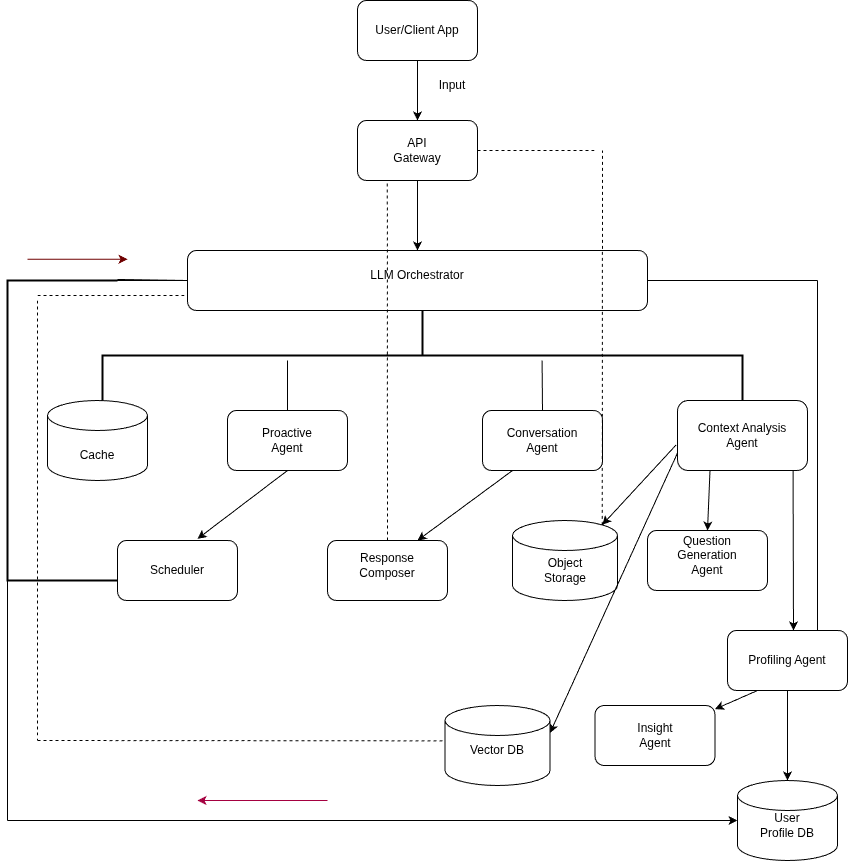
\includegraphics[scale=0.5]{design.png}
	\caption{High Level Design}
	\label{fig:high}
\end{figure}
	
\subsection{System Components}
\subsubsection{API Gateway}
Built using \texttt{FastAPI}, handling JWT authentication and serving as the interface for \textbf{Object Storage (S3)} uploads.

\subsubsection{LLM Orchestrator}
Implemented using \texttt{LangGraph} to manage state across specialized agents, utilizing \textbf{Redis} for Short-Term Memory (STM).

\subsubsection{Specialized Agents}
\begin{itemize}
	\item \textbf{Profiling Agent (PA):} Updates the \textbf{User Profile DB} with learner traits.
	\item \textbf{Content Analysis Agent (CAA):} Parses documents and stores embeddings in the \textbf{Vector DB}.
	\item \textbf{Question Generation Agent (QGA):} Creates assessments based on VDB context.
\end{itemize}

\section{Data Layer}
The system uses \textbf{PostgreSQL} for persistent profiles, \textbf{Pinecone} for semantic search, and \textbf{Redis} for session caching.

\section{System Architecture }

\begin{figure}[htbp]
	\centering
	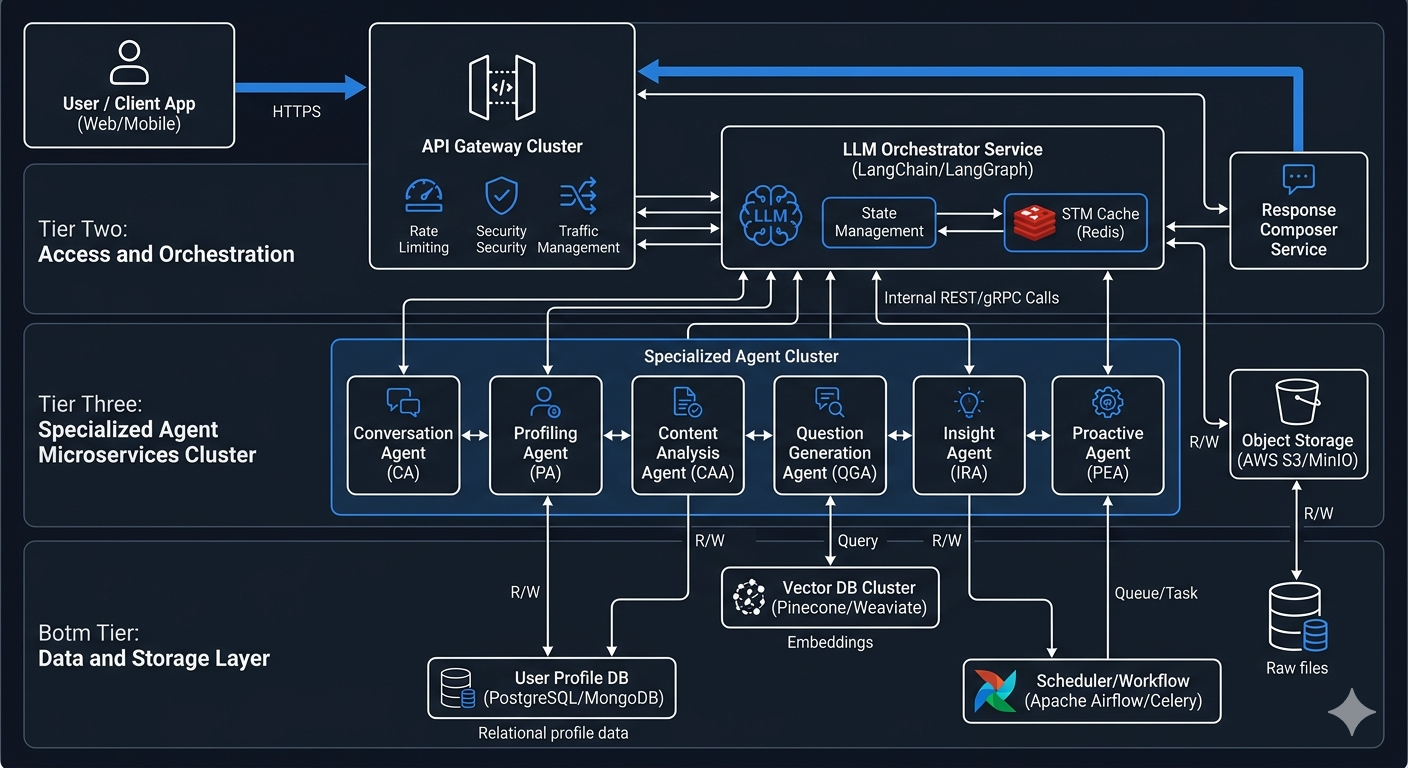
\includegraphics[scale=0.25]{arch.png}
	\caption{System Architecture}
	\label{fig:arch}
\end{figure}

%\section{Use-case Diagram }

%\section{Class Diagram}

%\section{Sequence Diagram}
%Include the Sequence diagram with respect to your project work

\chapter{Implementation}
%Some Introduction
\section{Overview of Technologies Used}
\section{Implementation details of modules}
\section{Challenges encountered and Strategies used to tackle}

%\chapter{Testing and Experimental Analysis and Results}
\section{Unit Testing}
\section{Integration Testing}
\section{Experimental Dataset}
\section{Performance Analysis}
	
%\chapter{Conclusion and Future Work}
% Future Work

\chapter{Summary}

The Two Sigma Problem is seen as the pinnacle of education, but as we’ve transitioned from traditional classrooms to modern LLMs, the experience is surprisingly fragmented. We have built tools that are powerful yet suffer from context drift, often forgetting a student’s specific struggles the moment a session ends. This survey reveals that while Multi-Agent Systems and LLMs have opened new doors, the real challenge lies in bridging the gap between AI and the user. By addressing the \enquote{forgetfulness} of current models, we try to improve the interaction between user and the machine, helping the user understand concepts without losing valuable instruction.

\clearpage
% ----- References -----
%\chapter*{REFERENCES}
%\addcontentsline{toc}{chapter}{REFERENCES}
%\begin{thebibliography}{99}
%	\bibitem{Rida2025} Z. Rida et al., "Dynamic Adaptation in an Intelligent Multi-Tutoring System: A Multi-Agent Approach," in \textit{IEEE Access}, vol. 13, 2025.
%	\bibitem{Hasan2020} M. A. Hasan et al., "The Transition From Intelligent to Affective Tutoring System: A Review and Open Issues," in \textit{IEEE Access}, vol. 8, 2020.
%	\bibitem{Zhang2025} Z. Zhang et al., "SPP-L2: A PPO-Enhanced LLM Framework for Student Performance Prediction," in \textit{IEEE Access}, vol. 13, 2025.
%	\bibitem{Hewedy2025} D. W. Hewedy and A. S. Abdelhady, "PETRA: A Personalized Educational Tutoring Tool," in \textit{Proc. ICEENG}, 2025.
%	\bibitem{Chaturvedi2026} N. Chaturvedi and A. Gunawardena, "Agentic Orchestration for Adaptive Educational Recommendations," in \textit{Proc. ACM WSDM}, 2026.
%	\bibitem{bloom} B. S. Bloom,  "The 2 Sigma Problem: The Search for Methods of Group Instruction as Effective as One-to-One Tutoring", in \textit{Educational Researcher}, 1984.
%\end{thebibliography}
\printbibliography[heading=bibintoc, title={REFERENCES}]
\clearpage

%% ----- Appendices -----
\appendix
\renewcommand{\thechapter}{\Alph{chapter}}
\renewcommand{\thesection}{\Roman{section}}
\section {Appendix A: Snapshots}
\clearpage
\section {Appendix B: Details of list of publications related to this project}
\large{Author Names: } \\
\large{Paper Title: } \\
\large {Name of the Conference or Journal:} \\
\large {Place of the conference:}\\ 
\large {Date of Conference:}
\clearpage
\section {Appendix C: Details of Patent}
\clearpage
\section {Appendix D: Details of Funding}
\clearpage

\section {Appendix E:POs and PSOs Mapped}
{\textcolor{red}{This is a  sample justification included you need to change as per your project}}
\begin{table}[h!]
	\centering
	\renewcommand{\arraystretch}{1.3} % Row height
	\setlength{\tabcolsep}{6pt}       % Column spacing
	\begin{tabular}{|p{3cm}|c|p{8cm}|}
		\hline
		\textbf{PROGRAMME OUTCOMES} & \textbf{Level (1/2/3)} & \textbf{Justification if addressed} \\
		\hline
		PO1 & 3 & The project applies engineering knowledge, including AI and ML principles, for detecting AI-generated code. \\
		\hline
		PO2 & 3 & Identifies and analyzes the issue of distinguishing AI generated code from human code using advanced research methods. \\
		\hline
		PO3 & 3 & Designs a comprehensive solution for AI code detection, integrating seamless feedback mechanisms into coding platforms. \\
		\hline
		PO4 & 3 & Conducts thorough research and experimentation using datasets to refine the AI verification model. \\
		\hline
		PO5 & 3 & Employs modern tools like TensorFlow, OpenAI APIs, and other NLP-based libraries to develop the system. \\
		\hline
		PO6 & 2 & Addresses societal needs by promoting fair assessments and reducing misuse of AI in coding evaluations. \\
		\hline
		PO7 & 1 & The project indirectly contributes to sustainable technology by promoting responsible use of AI in coding. \\
		\hline
		PO8 & 3 & Ensures ethical practices by encouraging transparency in AI generated code detection results. \\
		\hline
		PO9 & 3 & The project is developed collaboratively by a team, ensuring effective teamwork and contribution from all members. \\
		\hline
		PO10 & 2 & Prepares clear documentation and outputs for ease of use by academic institutions, recruiters, and developers. \\
		\hline
		PO11 & 2 & Demonstrates efficient resource management, including cloud hosting and API usage within a cost-effective budget. \\
		\hline
	\end{tabular}
	\caption{Programme Outcomes Mapping with Project}
\end{table}

\begin{table}[h!]
	\centering
	\renewcommand{\arraystretch}{1.3} % Row height
	\setlength{\tabcolsep}{6pt}       % Column spacing
	\begin{tabular}{|p{3cm}|c|p{8cm}|}
		\hline
		\textbf{PROGRAMME SPECIFIC OUTCOMES} & \textbf{Level (1/2/3)} & \textbf{Justification if addressed} \\
		\hline
		PSO1 & 1 & Minimal focus on computer networks; however, the project uses cloud hosting (e.g., DigitalOcean) for deployment. \\
		\hline
		PSO2 & 3 & Applies advanced software engineering practices and AI techniques to solve real-world code detection problems. \\
		\hline
		PSO3 & 3 & Integrates AI, NLP, and information systems to provide efficient and scalable solutions for technical evaluation. \\
		\hline
	\end{tabular}
	\caption{Programme Specific Outcomes Mapping with Project}
\end{table}
\clearpage

\section {Appendix F: Similarity report, AI Generated report}
\clearpage




\end{document}



